\documentclass{article}

% NeurIPS preprint style (no line numbers, author names shown, "Preprint" footer)
\usepackage[preprint]{neurips_2024}

% Standard packages
\usepackage{amsmath,amssymb}
\usepackage{booktabs}
\usepackage{graphicx}
\usepackage{hyperref}
\usepackage{url}
\usepackage{xcolor}
\usepackage{multirow}
\usepackage{nicefrac}

% Figure path
\graphicspath{{../figures/}}

% Hyperref styling
\hypersetup{
  colorlinks=true,
  linkcolor=blue!60!black,
  citecolor=blue!60!black,
  urlcolor=blue!60!black,
}

% Tight table spacing helper
\newcommand{\ra}[1]{\renewcommand{\arraystretch}{#1}}

\title{Epistemic Uncertainty in Language Models}

\author{
  Oleksiy Dolgykh \\
  \texttt{alexey.dolgich@gmail.com}
}

\begin{document}

\maketitle

% ============================================================================
\begin{abstract}
We present a comparison of four Bayesian approaches to epistemic uncertainty estimation in language models, organized as a $2{\times}2$ matrix: (variational vs.\ post-hoc) $\times$ (full weights vs.\ LoRA adapters), plus an MC Dropout baseline. All methods are evaluated on the same 76M-parameter GPT-2-style architecture trained on The Pile with domain-split OOD evaluation. We report three main findings.
First, \textbf{LoRA-based Bayesian methods achieved the strongest OOD detection in our setup}: BLoB LoRA (AUROC 0.909) and TFB (0.917) outperform full-weight variational inference (0.874) with $17{\times}$ fewer Bayesian parameters, though this comparison is confounded by differences in training procedure and backbone quality (\S\ref{sec:discussion}).
Second, \textbf{diagonal Laplace approximation fails} for language model OOD detection---the diagonal Fisher curvature is flat at convergence regardless of parameterization (full weights or LoRA).
Third, \textbf{MC Dropout} applied to the deterministic checkpoint (zero extra training) achieves AUROC 0.898---surprisingly competitive with trained Bayesian methods (overlapping confidence intervals with BLoB).
\textbf{TFB}, also requiring no Bayesian training, matches the best trained methods at AUROC 0.917.
Production benchmarks show $N{=}3$ MC samples capture 97\% of the full signal at 50\,ms per sequence.
\end{abstract}

% ============================================================================
\section{Introduction}
\label{sec:introduction}

Large language models produce confident predictions even on inputs far from their training distribution. Standard softmax probabilities conflate two distinct sources of uncertainty: \textbf{aleatoric} uncertainty (inherent ambiguity in the data) and \textbf{epistemic} uncertainty (what the model doesn't know). Distinguishing these is critical for safe deployment---a model should flag when it is uncertain due to lack of knowledge, not just when the next token is ambiguous.

Bayesian inference offers a principled framework: replace point-estimate weights with posterior distributions, then measure disagreement across weight samples. Mutual information (MI) between weights and predictions isolates the epistemic component. High MI signals ``the model's weights disagree about this input''---a direct indicator of out-of-distribution data.

Recent work has introduced several practical methods for Bayesian weight posteriors in large models, including variational LoRA \citep[BLoB;][]{wang2024blob}, post-hoc SVD-based variance \citep[TFB;][]{shi2025training}, and post-hoc Laplace on LoRA \citep{yang2024bayesian}. However, these methods have been evaluated on different architectures, datasets, and metrics, making direct comparison impossible.

We address this gap with a \textbf{controlled $2{\times}2$ comparison} on a single architecture and evaluation protocol:

\begin{table}[h]
\centering
\small
\begin{tabular}{@{}lcc@{}}
\toprule
 & \textbf{Full weights} & \textbf{LoRA adapters} \\
\midrule
\textbf{Variational} (train-time) & Variational FFN & BLoB LoRA \\
\textbf{Post-hoc} (no Bayesian training) & Diag.\ Laplace FFN & TFB / Diag.\ Laplace LoRA \\
\bottomrule
\end{tabular}
\end{table}

\noindent All four cells are evaluated on the same 76M-parameter GPT-2-style model trained on The Pile with domain-split evaluation (in-distribution: HackerNews; OOD: ArXiv, FreeLaw, PubMed). We evaluate using AUROC, FPR@95, AUPRC, ECE, Brier score, NLL, and AURC, and report production inference costs.

\begin{figure}[t]
\centering
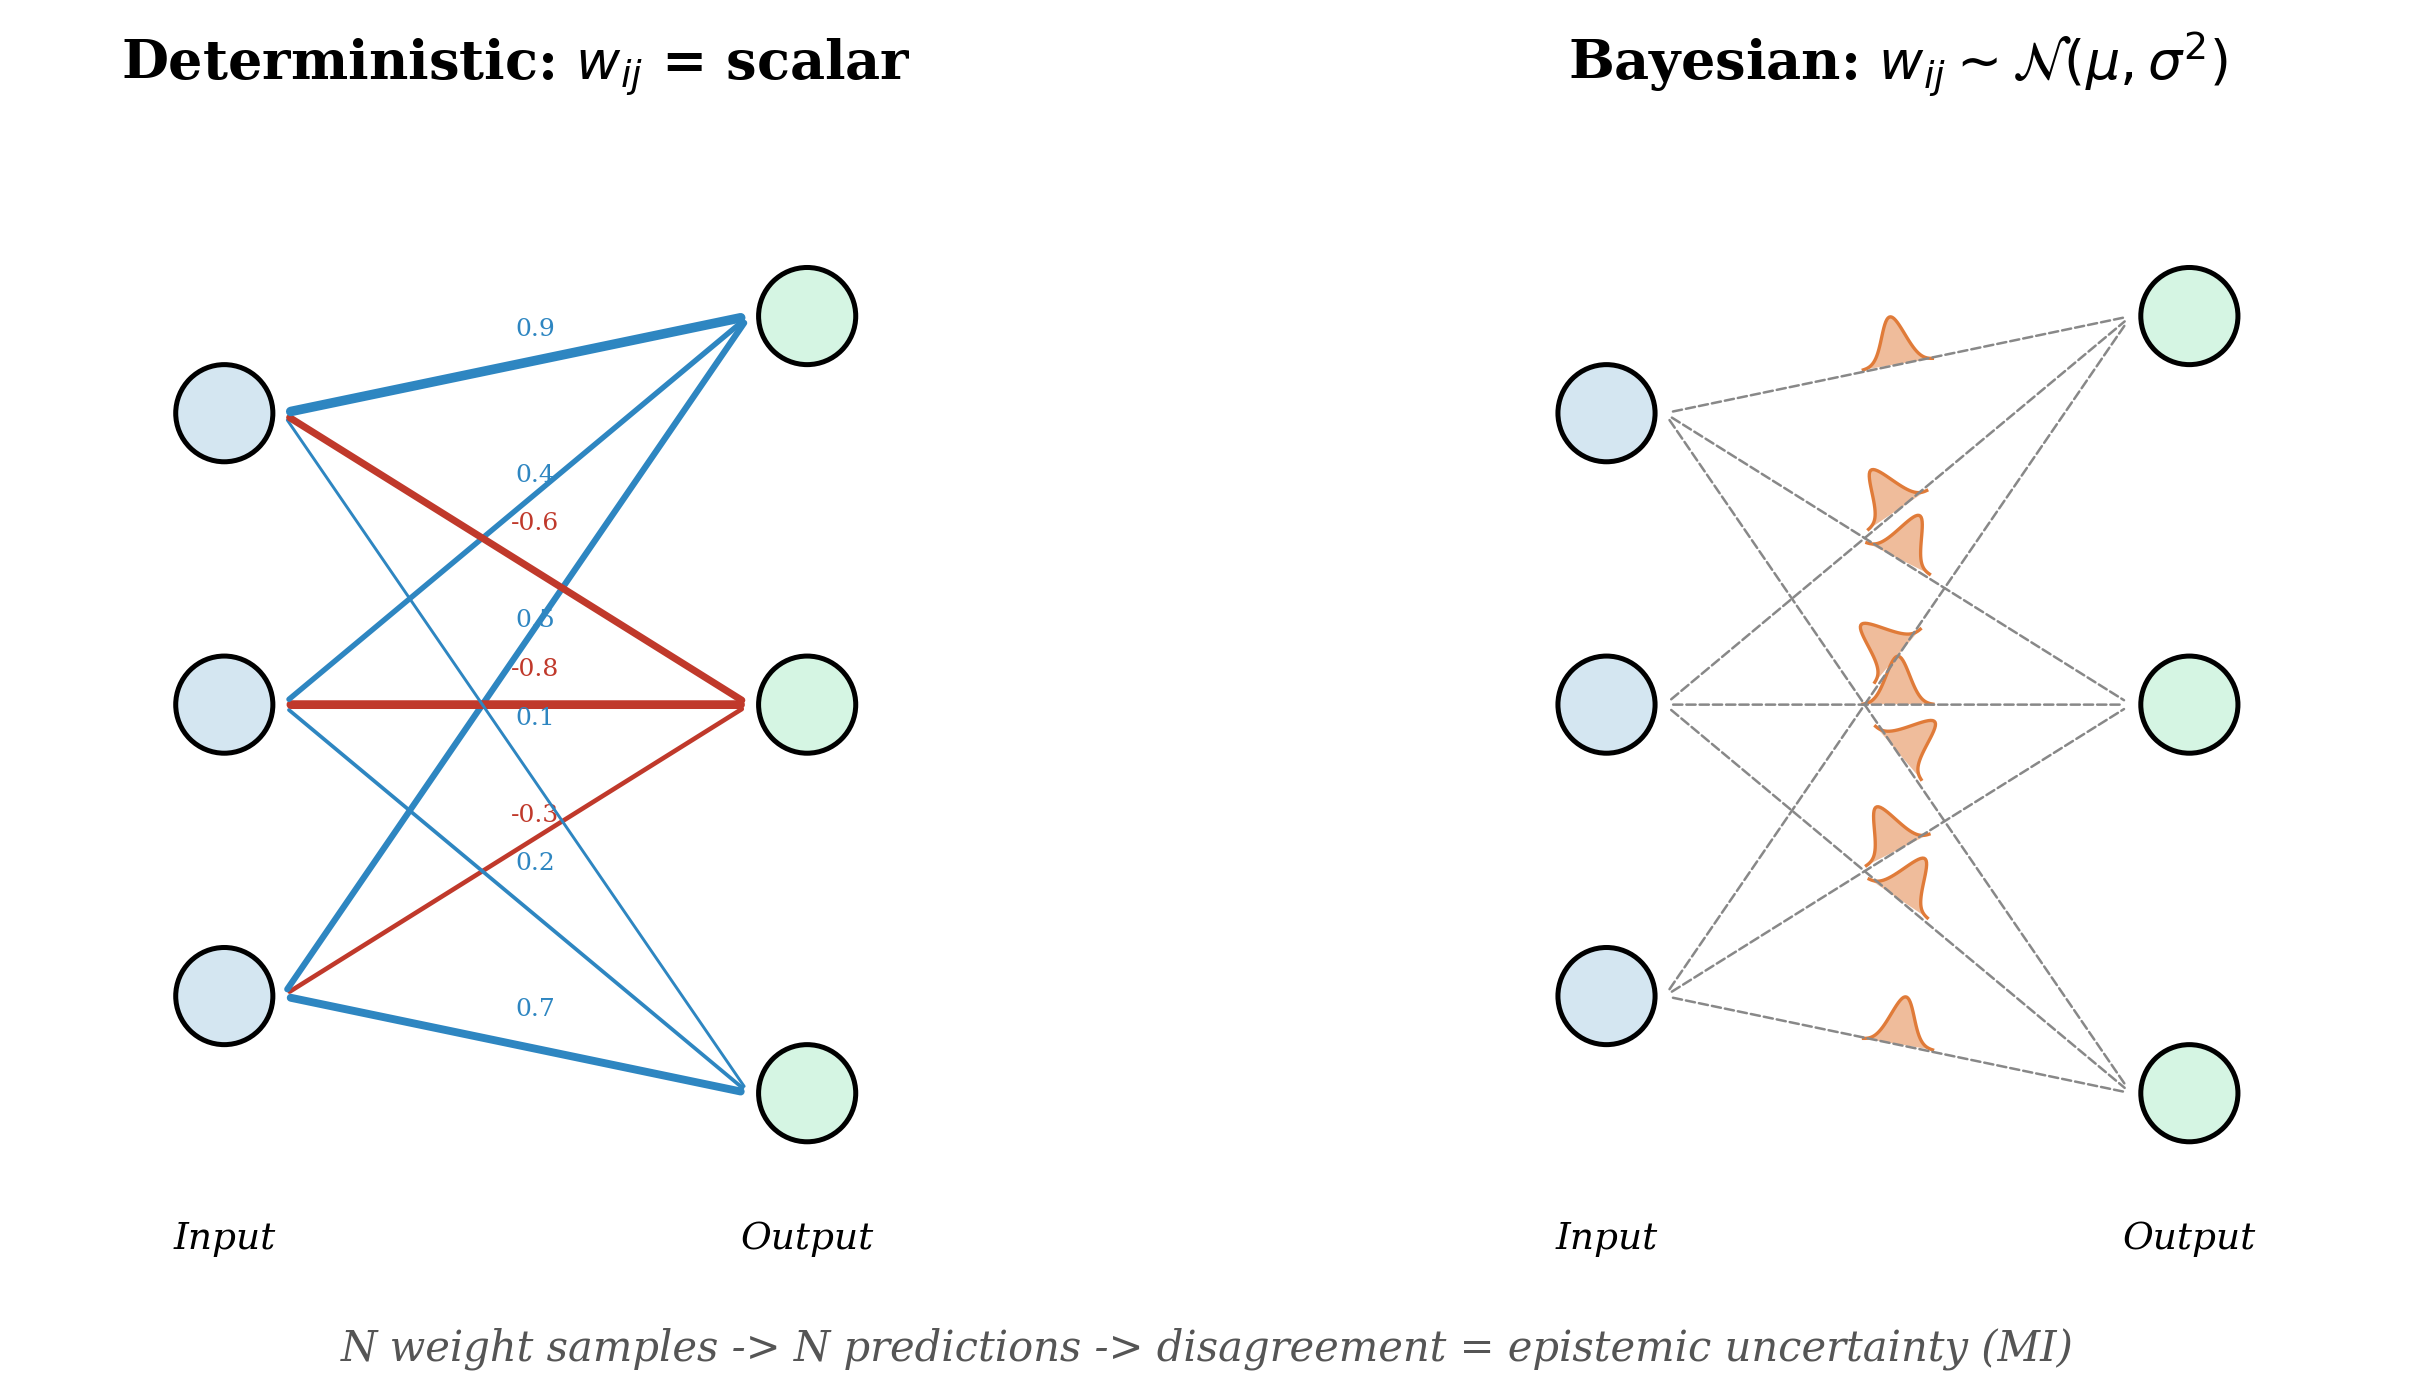
\includegraphics[width=0.85\textwidth]{fig1_point_vs_bayesian.png}
\caption{Point weights vs.\ Bayesian weight posteriors. Standard neural networks learn a single weight value (left); Bayesian approaches maintain a distribution over weights (right), enabling epistemic uncertainty estimation through prediction disagreement across weight samples.}
\label{fig:point-vs-bayesian}
\end{figure}

\paragraph{Contributions.}
\begin{enumerate}
\item First controlled head-to-head comparison of variational vs.\ post-hoc Bayesian methods on the same LM architecture, dataset, and evaluation protocol, including an MC Dropout baseline.
\item LoRA-based methods (BLoB, TFB) achieved stronger OOD detection than full-weight variational inference at 76M parameters, though the comparison is confounded by training procedure and backbone quality differences (\S\ref{sec:discussion}).
\item Definitive negative result for \textbf{diagonal Laplace} in LM OOD detection---both full-weight and LoRA parameterizations produce MI ratio $1.00{\times}$. This does not extend to KFAC or full-Hessian variants.
\item \textbf{MC Dropout} (zero extra training) achieves AUROC 0.898---a surprisingly strong baseline whose confidence interval overlaps with trained BLoB LoRA (0.909). \textbf{TFB} (also zero Bayesian training) achieves the best AUROC (0.917) via SVD-structured variance on existing LoRA checkpoints.
\item Production deployment recipe: merged mean-weights for serving (zero overhead vs.\ deterministic), $N{=}3$ MC for uncertainty scoring (97\% of full signal at 50\,ms/sequence).
\end{enumerate}

\begin{figure}[t]
\centering
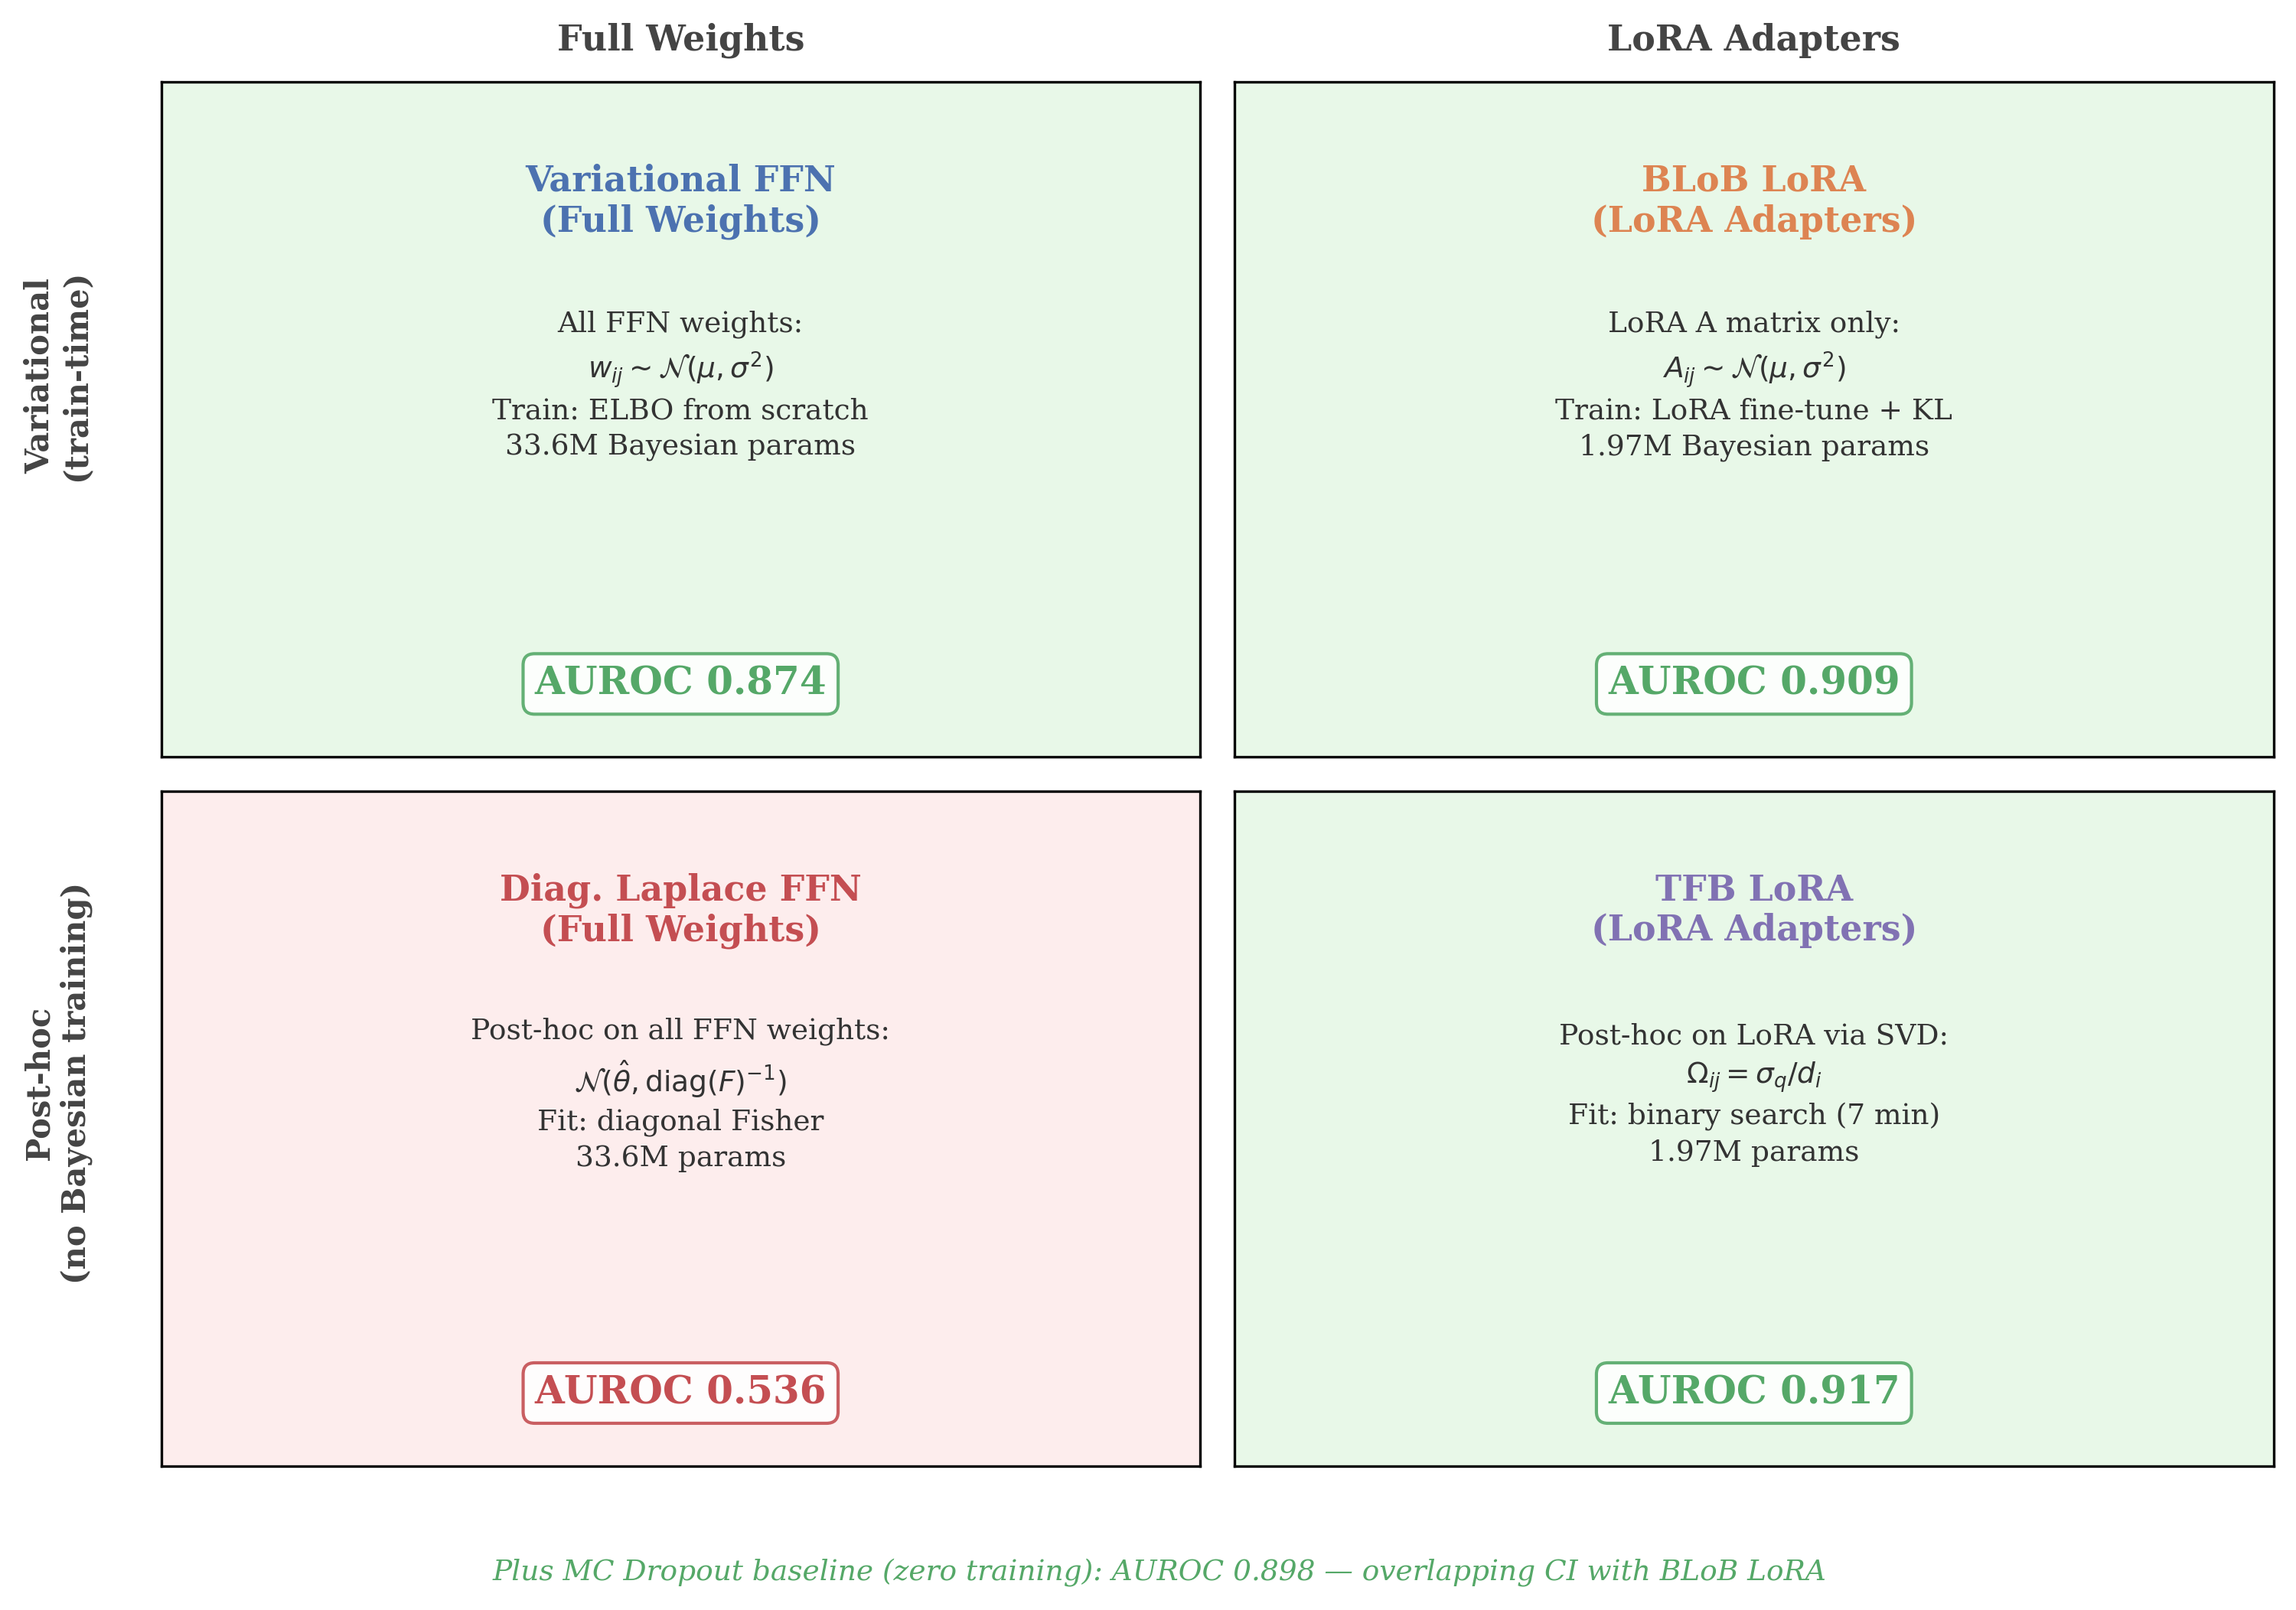
\includegraphics[width=0.9\textwidth]{fig2_method_matrix.png}
\caption{Four Bayesian methods evaluated in a $2{\times}2$ comparison at 76M parameters. Rows distinguish variational (train-time) from post-hoc (no Bayesian training) approaches; columns distinguish full-weight from LoRA parameterizations. AUROC values shown for OOD detection.}
\label{fig:method-matrix}
\end{figure}

% ============================================================================
\section{Related Work}
\label{sec:related}

\paragraph{Bayesian neural networks.}
Variational inference for neural network weights was introduced by \citet{graves2011practical} and scaled by \citet{blundell2015weight} with Bayes by Backprop. Flipout \citep{wen2018flipout} reduces gradient variance through pseudo-independent weight perturbations. These methods provide principled uncertainty but have historically been difficult to scale beyond small networks.

\paragraph{Laplace approximation.}
Post-hoc Laplace fits a Gaussian posterior at the MAP estimate using curvature information. \citet{daxberger2021laplace} systematized the approach with diagonal, KFAC, and full Hessian variants. While effective for image classifiers, diagonal Laplace has known limitations when Fisher curvature is flat---a condition we find is endemic to well-trained language models.

\paragraph{Bayesian LoRA methods.}
Low-Rank Adaptation \citep{hu2022lora} enables parameter-efficient fine-tuning. Several works extend LoRA with Bayesian posteriors. \textbf{BLoB} \citep{wang2024blob} places variational Gaussian posteriors on LoRA's $A$ matrix during training, using a KL decomposition theorem to avoid full-space computation. \textbf{TFB} \citep{shi2025training} converts trained LoRA checkpoints into Bayesian adapters post-hoc via SVD-structured isotropic variance with binary search calibration. \textbf{Laplace-LoRA} \citep{yang2024bayesian} applies Laplace approximation to LoRA parameters. \textbf{ScalaBL} \citep{samplawski2025scalable} performs Bayesian inference in the $r$-dimensional subspace defined by LoRA rank, scaling to 32B parameters.

These methods report results on different model families (LLaMA, Qwen, GPT-2), different tasks (MMLU, commonsense QA, calibration), and different metrics. Our contribution is a controlled apples-to-apples comparison on a single setup.

\paragraph{OOD detection in LMs.}
Most work uses token-level predictive entropy or energy scores. We focus on epistemic uncertainty via mutual information, which requires a weight posterior and is theoretically grounded in Bayesian decision theory.

% ============================================================================
\section{Methods}
\label{sec:methods}

\subsection{Uncertainty Quantification}

Given a model with weight posterior $q(\theta)$, we draw $N$ weight samples $\{\theta^{(i)}\}_{i=1}^N$ and compute token-level predictive distributions $p_t^{(i)} = \text{softmax}(f_{\theta^{(i)}}(x)_t)$. Epistemic uncertainty is measured by \textbf{mutual information} (MI):
\begin{equation}
\text{MI} = H\!\left[\frac{1}{N}\sum_{i=1}^{N} p_t^{(i)}\right] - \frac{1}{N}\sum_{i=1}^{N} H\!\left[p_t^{(i)}\right]
\label{eq:mi}
\end{equation}
The first term (predictive entropy) captures total uncertainty; the second (expected entropy) captures aleatoric uncertainty. Their difference isolates the epistemic component---uncertainty due to weight disagreement.

For OOD detection, we compute mean MI per sequence and threshold: high MI $\rightarrow$ OOD. We report AUROC as the primary metric, with FPR@95 as the production-relevant operating point.

\subsection{Variational Full-Weight}

Standard Bayes by Backprop applied to all FFN layers (fc and proj sublayers across all transformer blocks). Each weight $w_{ij}$ is parameterized as $\mathcal{N}(\mu_{ij}, \sigma_{ij}^2)$ with $\sigma_{ij} = \log(1 + \exp(\rho_{ij}))$. Training minimizes the ELBO: reconstruction loss plus KL divergence to a standard normal prior. This doubles the FFN parameter count (33.6M Bayesian parameters on a 76M model).

\subsection{BLoB LoRA}

Bayesian Low-Rank Adaptation by Backpropagation \citep{wang2024blob}. LoRA decomposes weight updates as $\Delta W = \frac{\alpha}{r} BA$, with rank $r{=}16$. BLoB places variational Gaussian posteriors on $A$ while keeping $B$ deterministic. Via a KL factorization theorem, the full-weight KL reduces to a diagonal computation in the low-rank $A$-space. Training uses Flipout for variance reduction. Total Bayesian parameters: 1.97M (2.5\% of model).

\begin{figure}[t]
\centering
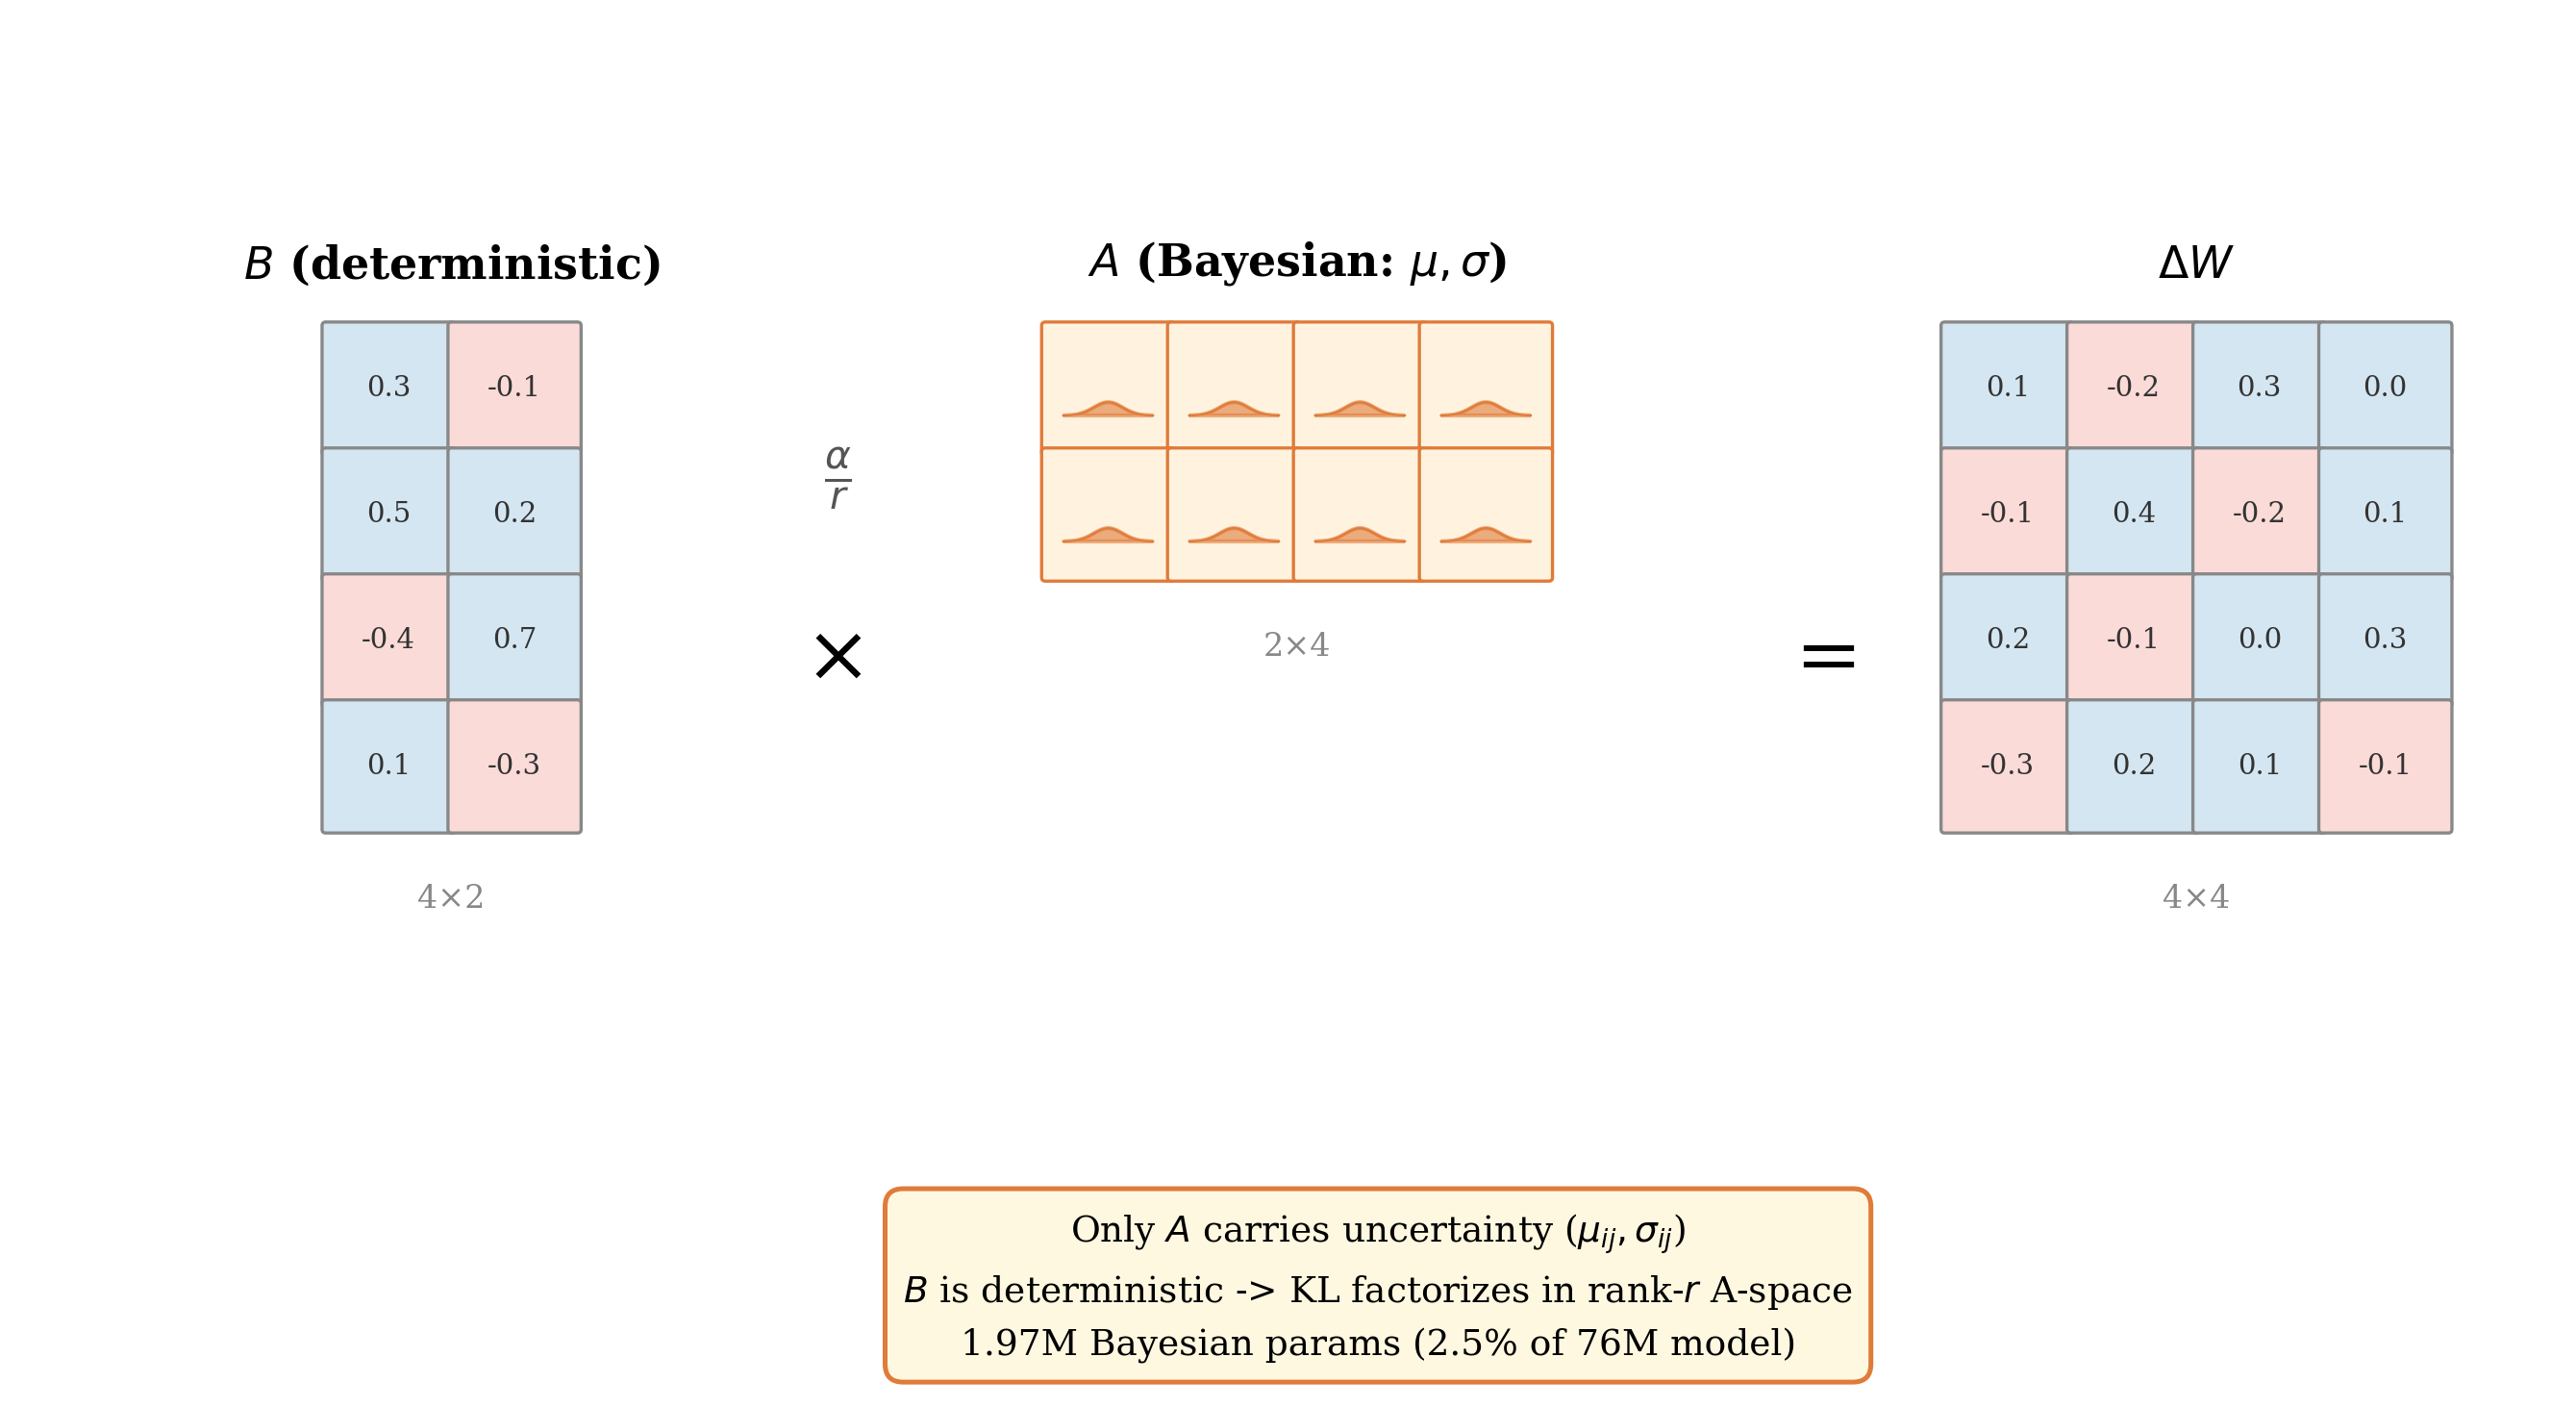
\includegraphics[width=0.85\textwidth]{fig3_blob_lora.png}
\caption{BLoB LoRA architecture. The $A$ matrix carries variational Gaussian posteriors ($\mu_A$, $\sigma_A$); the $B$ matrix remains deterministic. At inference, $N$ weight samples from $A$ produce $N$ predictions whose disagreement (MI) measures epistemic uncertainty.}
\label{fig:blob-lora}
\end{figure}

\subsection{Diagonal Laplace Approximation}

Post-hoc diagonal Laplace: fit a Gaussian posterior $\mathcal{N}\!\left(\hat{\theta},\, (\text{diag}(F) + \lambda I)^{-1}\right)$ at the MAP estimate using per-sample diagonal Fisher information. Applied to both full FFN weights (33.6M parameters) and LoRA parameters (1.97M parameters). No Bayesian training---operates on existing deterministic or LoRA checkpoints.

\subsection{TFB}

Training-Free Bayesianization \citep{shi2025training}. Converts a trained LoRA checkpoint into a Bayesian adapter without retraining. SVD of $B$ yields singular values that define per-direction variance scaling: $\Omega_{ij} = \sigma_q / d_i$, where $d_i$ are singular values. A single scalar $\sigma_q$ controls the posterior width, found by binary search on a calibration set. Total fit time: 7 minutes.

\subsection{MC Dropout}

Monte Carlo Dropout \citep{gal2016dropout} interprets dropout at inference as approximate variational inference with a Bernoulli posterior over weights---each dropout mask corresponds to a sample from this posterior. We apply it to the deterministic baseline checkpoint (C0) with the training dropout rate (0.1) on attention and FFN dropout layers. At inference, $N$ stochastic forward passes (each with a different random dropout mask) produce $N$ predictions; MI is computed from their disagreement. No retraining or architectural changes are required---MC Dropout can be applied to any model that was trained with dropout.

% ============================================================================
\section{Experimental Setup}
\label{sec:setup}

\paragraph{Architecture.}
GPT-2-style transformer: 16 layers, 8 heads, 512 embedding dimension, 2048 FFN width. ${\sim}$76M parameters. No modern tricks (RoPE, SwiGLU, GQA)---deliberately minimal to isolate Bayesian effects from architecture improvements.

\paragraph{Dataset.}
The Pile \citep{gao2020pile}, domain-split for OOD evaluation. Training domains: StackExchange, Ubuntu IRC, EuroParl, HackerNews. OOD domains: ArXiv, FreeLaw, PubMed Central. BPE tokenization (GPT-2 vocabulary, 50{,}257 tokens). Training: ${\sim}$100K steps, batch size 16, sequence length 256.

\paragraph{Evaluation protocol.}
500 in-distribution sequences (HackerNews) and 500 OOD sequences (ArXiv + FreeLaw + PubMed) at block\_size=256. $N{=}20$ MC weight samples (or dropout passes for MC Dropout). Metrics: AUROC, FPR@95 TPR, AUPRC, ECE, Brier score, NLL, AURC. Each Bayesian method uses MI as its uncertainty score; the deterministic baseline uses max-probability. MC Dropout uses the deterministic checkpoint with dropout enabled at inference. 95\% bootstrap CIs (10{,}000 resamples) are reported for AUROC.

\paragraph{Hardware.}
Single NVIDIA RTX 4070 (12\,GB VRAM). AMP fp16 enabled. PyTorch~2.x with Flash Attention.

% ============================================================================
\section{Results}
\label{sec:results}

\subsection{OOD Detection}

\begin{table}[t]
\caption{OOD detection performance (16L scale, 500 ID + 500 OOD sequences, $N{=}20$ MC samples). Bold indicates best result per column among Bayesian methods. 95\% bootstrap CIs from 10{,}000 resamples.}
\label{tab:ood}
\centering
\footnotesize
\ra{1.15}
\setlength{\tabcolsep}{4pt}
\begin{tabular}{@{}llccccccc@{}}
\toprule
Method & Type & MI & AUROC [95\% CI] & FPR@95 & AUPRC & ECE & Brier & NLL \\
\midrule
Deterministic & --- & --- & .591\,[.556,\,.626] & .794 & .552 & .022 & .606 & 2.79 \\
MC Dropout & --- & --- & .898\,[.877,\,.917] & .368 & .870 & \textbf{.012} & .608 & \textbf{2.79} \\
\midrule
Var.\ FFN & Var\,$\times$\,Full & 1.32$\times$ & .874\,[.852,\,.895] & .494 & .866 & .023 & .673 & 3.31 \\
Diag.\ Lap.\ FFN & Post\,$\times$\,Full & 1.00$\times$ & .536\,[.500,\,.572] & .934 & .533 & .033 & 1.00 & 9.10 \\
\textbf{BLoB LoRA} & \textbf{Var\,$\times$\,LoRA} & \textbf{1.53$\times$} & \textbf{.909}\,[.890,\,.925] & .424 & .909 & .044 & .658 & 3.06 \\
\textbf{TFB LoRA} & \textbf{Post\,$\times$\,LoRA} & 1.35$\times$ & \textbf{.917}\,[.900,\,.933] & \textbf{.384} & \textbf{.918} & .022 & .658 & 3.06 \\
Diag.\ Lap.\ LoRA & Post\,$\times$\,LoRA & 1.00$\times$ & .494\,[.459,\,.529] & .956 & .495 & .034 & .998 & 9.73 \\
\bottomrule
\end{tabular}
\end{table}

\begin{figure}[t]
\centering
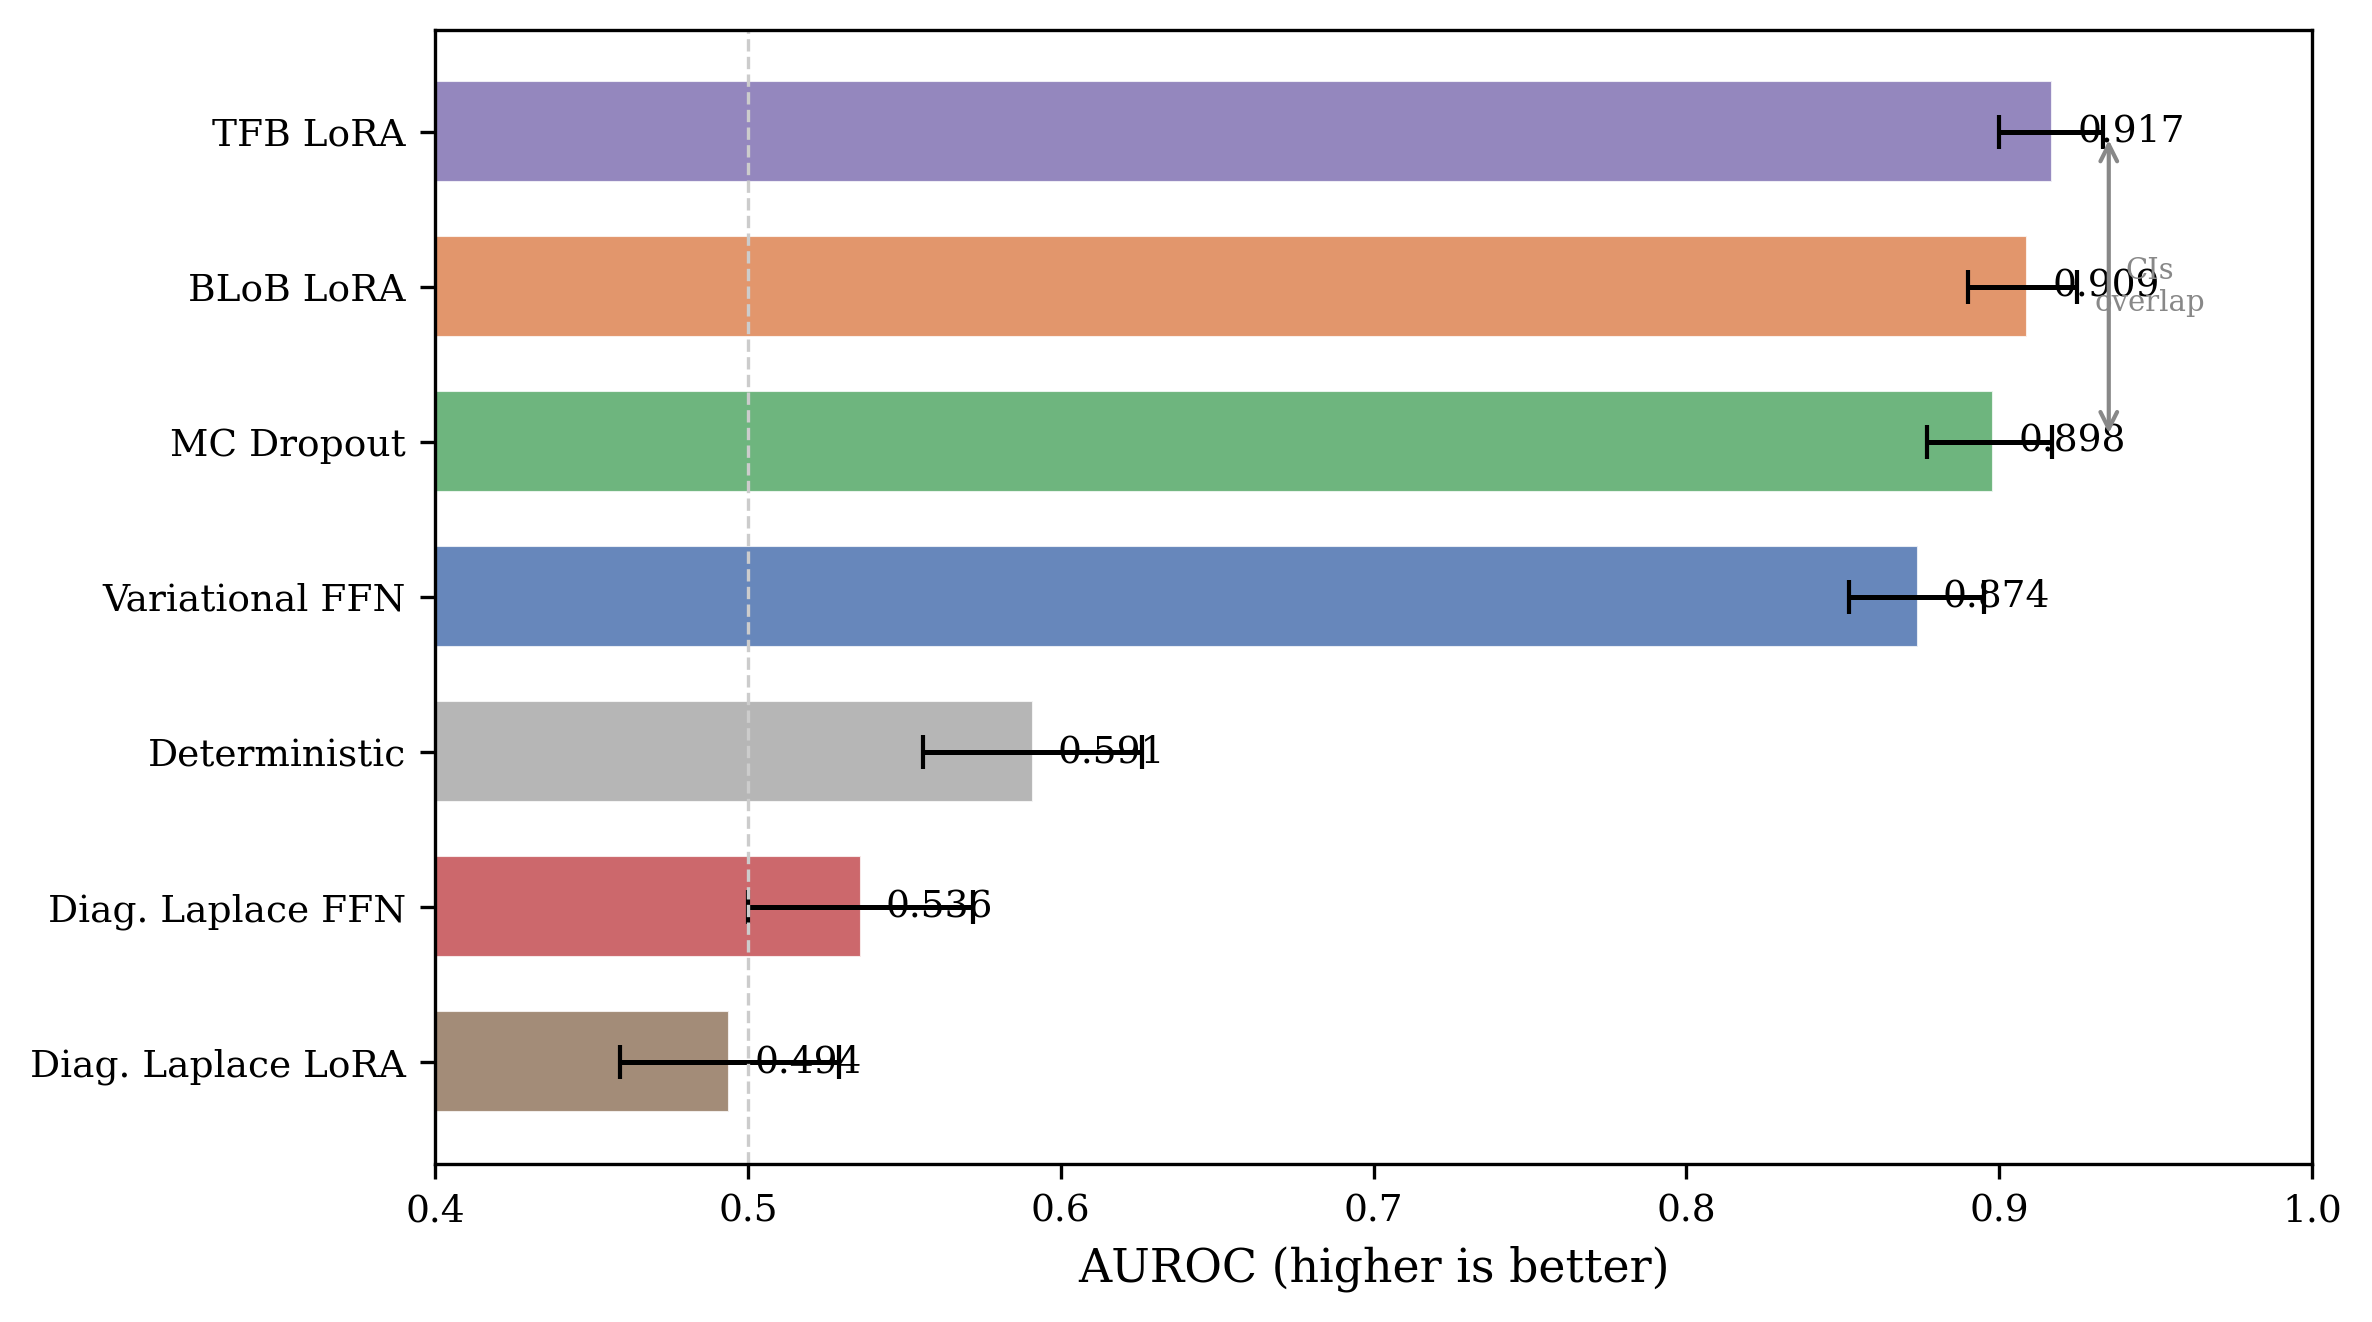
\includegraphics[width=0.85\textwidth]{fig5_auroc_bars.png}
\caption{OOD detection AUROC with 95\% bootstrap confidence intervals ($n{=}10{,}000$ resamples). TFB and BLoB LoRA lead with overlapping CIs; MC Dropout (zero training cost) is surprisingly competitive. Both diagonal Laplace variants are near-random.}
\label{fig:auroc-bars}
\end{figure}

The two LoRA methods---BLoB (variational) and TFB (post-hoc)---achieve the strongest OOD detection (AUROC 0.909 and 0.917, with overlapping 95\% bootstrap CIs). MC Dropout, a zero-training baseline applied to the deterministic checkpoint, is surprisingly competitive at AUROC 0.898 with the best calibration (ECE=0.012). Full-weight variational inference reaches 0.874 but requires $17{\times}$ more Bayesian parameters than LoRA methods. Both diagonal Laplace variants produce near-random OOD detection (AUROC $\approx 0.5$) with severely degraded calibration (Brier $\approx 1.0$, NLL $> 9.0$). All 95\% CIs are computed via 10{,}000 bootstrap resamples of per-sequence scores.

MI is the only effective uncertainty score. Predictive entropy and max-probability AUROC remain near 0.5 for all methods (Table~\ref{tab:score-comparison}), confirming that token-level uncertainty is insufficient for OOD detection---weight-level disagreement (MI) is required.

\begin{table}[t]
\caption{Uncertainty score comparison (AUROC by score type). MI provides effective OOD discrimination; predictive entropy and max-probability do not.}
\label{tab:score-comparison}
\centering
\small
\ra{1.15}
\begin{tabular}{@{}lccc@{}}
\toprule
Method & MI & Pred.\ Entropy & Max-Prob \\
\midrule
Deterministic & --- & 0.545 & 0.591 \\
MC Dropout & 0.898 & 0.561 & 0.615 \\
Variational FFN & 0.874 & 0.506 & 0.548 \\
BLoB LoRA & 0.909 & 0.532 & 0.569 \\
TFB LoRA & \textbf{0.917} & 0.553 & 0.589 \\
\bottomrule
\end{tabular}
\end{table}

\paragraph{Key takeaways from Table~\ref{tab:ood}.}
(1)~MC Dropout---a zero-cost Bayesian baseline requiring no extra training---achieves AUROC 0.898, surprisingly competitive with trained methods. Its 95\% CI [0.877, 0.917] overlaps with BLoB LoRA [0.890, 0.925], so the advantage of trained variational LoRA over MC Dropout is not statistically significant at this sample size. Practitioners should consider whether the modest AUROC gain justifies the additional training cost.
(2)~MC Dropout achieves the best calibration (ECE=0.012) and tied-lowest NLL (2.79), suggesting that dropout's implicit regularization benefits prediction quality alongside uncertainty estimation.
(3)~Diagonal Laplace is definitively negative---the result is consistent across four independent experiments (B1, B3-LAP, C2, C4-LAP), two scales (4L, 16L), and both parameterizations (full weights, LoRA).
(4)~TFB (AUROC 0.917, also zero Bayesian training) is the strongest single method, though its CI overlaps with both BLoB and MC Dropout.

\subsection{Production Viability}

\begin{table}[t]
\caption{Inference benchmarks (RTX 4070, sequence length 256, batch size 1, AMP fp16). Overhead is relative to deterministic baseline. LoRA MC uses 28\% less VRAM than full variational MC.}
\label{tab:inference}
\centering
\small
\ra{1.15}
\begin{tabular}{@{}lcccc@{}}
\toprule
Method & $N$ & Latency (ms) & Overhead & VRAM (MB) \\
\midrule
Deterministic & 1 & 8.1 & 1.0$\times$ & 470 \\
Full Var.\ MC & 5 & 71.0 & 8.8$\times$ & 534 \\
Full Var.\ MC & 20 & 286.9 & 35.4$\times$ & 534 \\
BLoB LoRA MC & 3 & 50.5 & 6.2$\times$ & 382 \\
BLoB LoRA MC & 5 & 84.4 & 10.4$\times$ & 382 \\
TFB LoRA MC & 5 & 133.0 & 16.4$\times$ & 389 \\
\bottomrule
\end{tabular}
\end{table}

Each MC sample requires a full forward pass because the residual stream diverges after each Bayesian FFN layer---there is no shared computation to amortize. Overhead scales linearly with $N$. LoRA MC uses 28\% less VRAM than full variational MC (382 vs.\ 534\,MB) because only 2.5\% of parameters carry variance.

\begin{table}[t]
\caption{AUROC vs.\ number of MC samples $N$ (200 ID + 200 OOD sequences). $N{=}3$ captures ${\sim}97\%$ of the $N{=}20$ signal for all methods.}
\label{tab:n-vs-auroc}
\centering
\small
\ra{1.15}
\begin{tabular}{@{}lccccc@{}}
\toprule
Method & $N{=}1$ & $N{=}3$ & $N{=}5$ & $N{=}10$ & $N{=}20$ \\
\midrule
Full Var.\ MC & 0.500 & 0.850 & 0.855 & 0.866 & 0.869 \\
BLoB LoRA MC & 0.500 & \textbf{0.861} & \textbf{0.879} & 0.880 & 0.888 \\
TFB LoRA MC & 0.500 & 0.847 & 0.859 & 0.881 & 0.886 \\
\bottomrule
\end{tabular}
\end{table}

\begin{figure}[t]
\centering
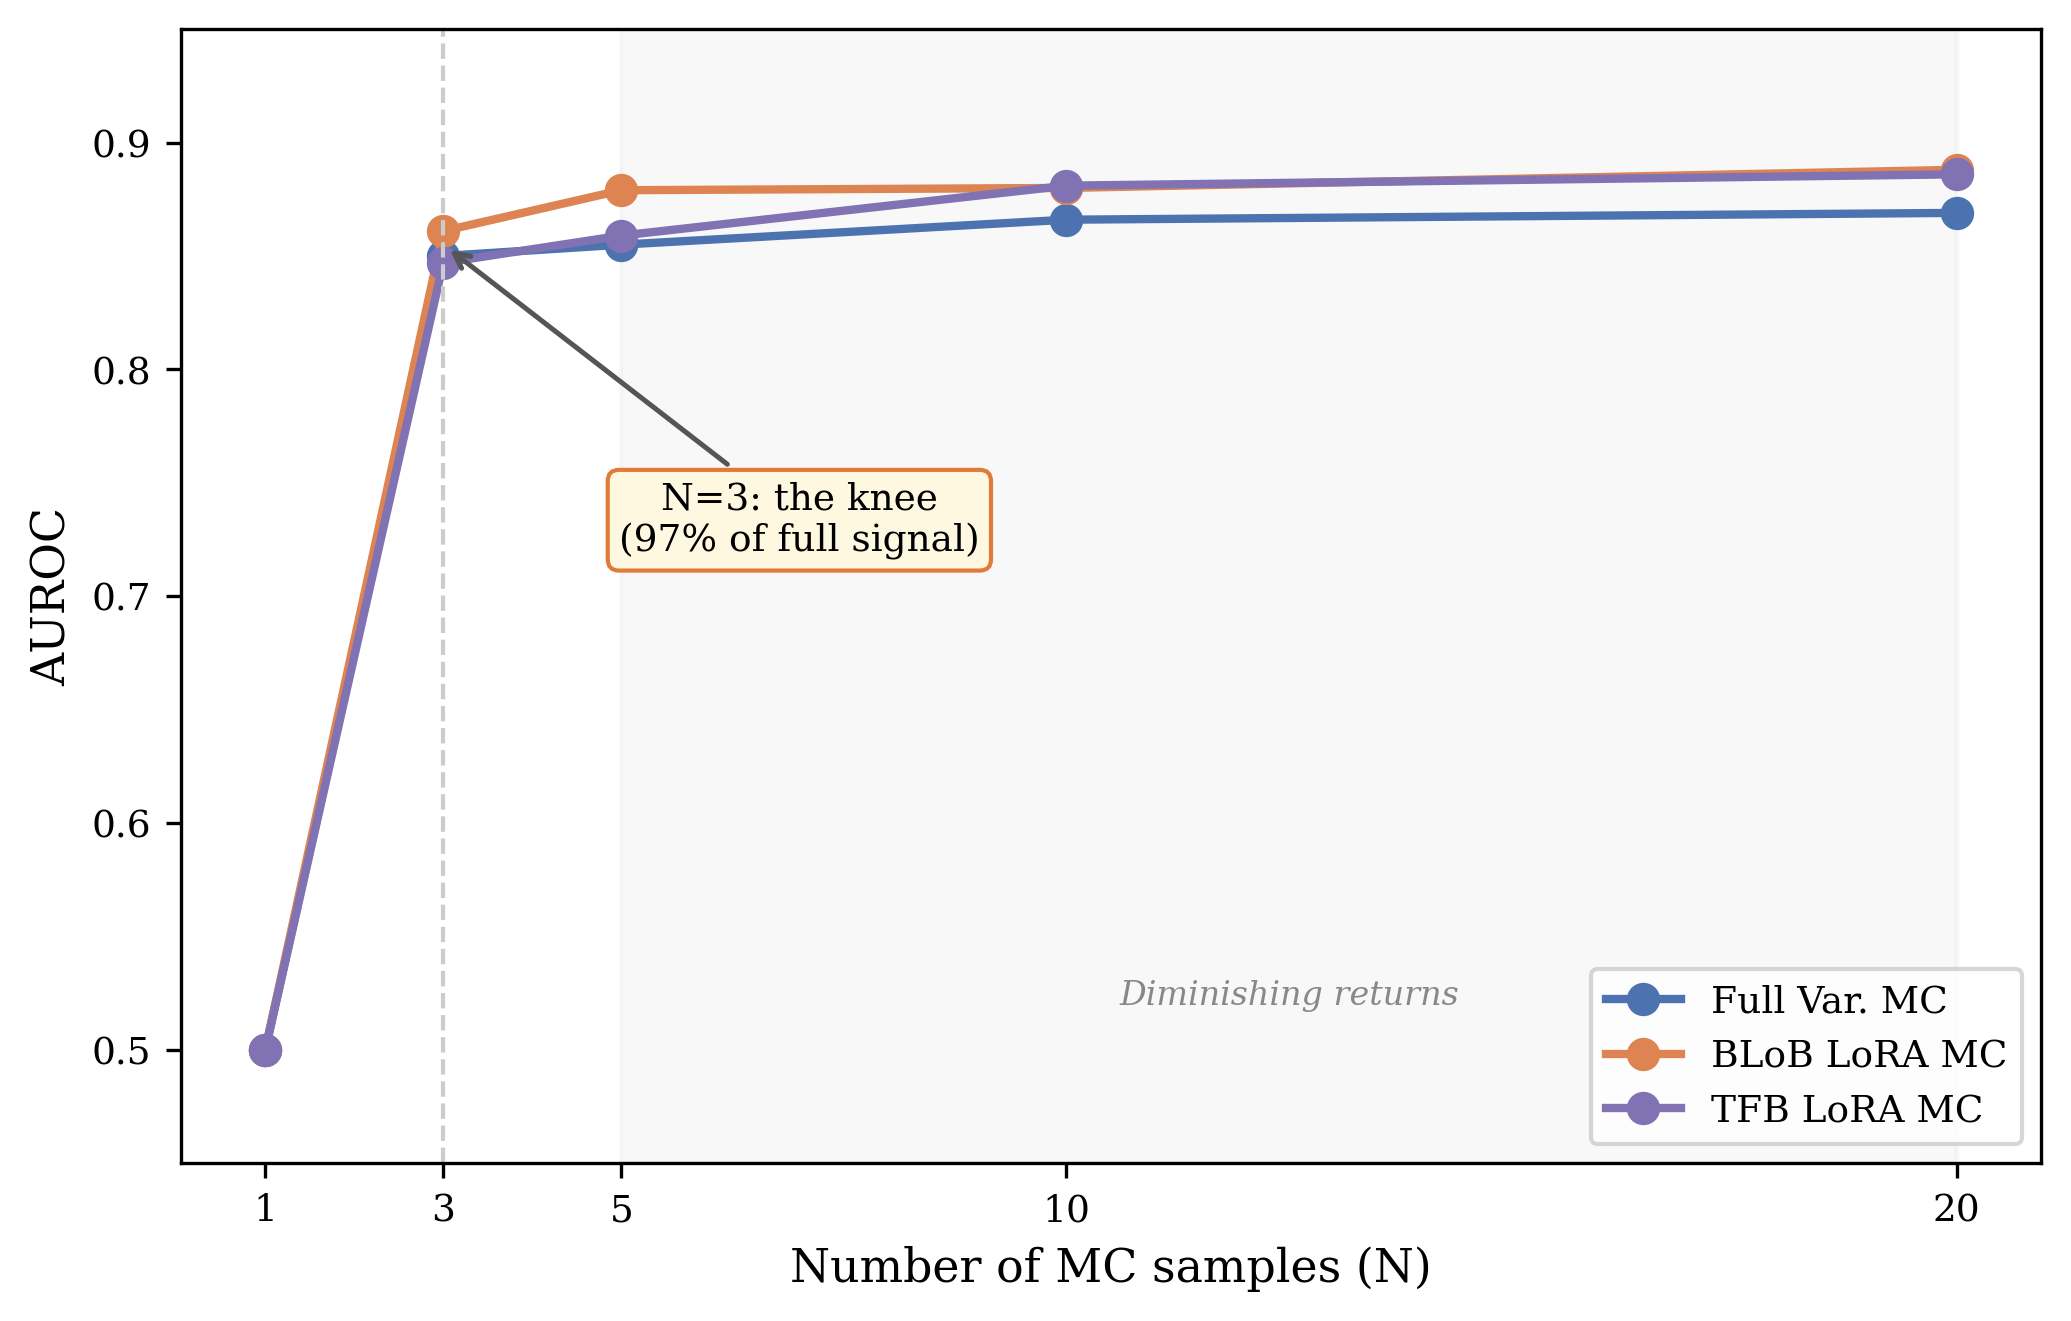
\includegraphics[width=0.75\textwidth]{fig6_n_vs_auroc.png}
\caption{AUROC vs.\ number of MC samples. $N{=}3$ is the knee: AUROC jumps from 0.50 ($N{=}1$, no disagreement possible) to ${\sim}$0.86 ($N{=}3$)---97\% of the $N{=}20$ signal. Further samples add diminishing returns.}
\label{fig:n-vs-auroc}
\end{figure}

\paragraph{$N{=}3$ is the knee.}
AUROC jumps from 0.50 ($N{=}1$, no disagreement possible) to ${\sim}$0.86 ($N{=}3$)---97\% of the $N{=}20$ signal. Further samples add diminishing returns: $N{=}5 \to 20$ contributes $<$3 AUROC points. The production sweet spot is \textbf{$N{=}3$ at 50\,ms/sequence with 382\,MB VRAM}.

\subsection{Mean-Weights Inference}

For serving predictions (without uncertainty scoring), mean-weights inference uses the posterior mean $\mu$ as a deterministic point estimate. This avoids MC sampling entirely.

\begin{table}[t]
\caption{Mean-weights PPL vs.\ MC-averaged PPL ($N{=}20$). Mean-weights matches MC-averaged within 4\%, enabling zero-overhead serving.}
\label{tab:mean-weights}
\centering
\small
\ra{1.15}
\begin{tabular}{@{}lccc@{}}
\toprule
Method & Mean-Wt PPL & MC-Avg PPL & Relative Diff \\
\midrule
Variational FFN & 24.48 & 24.41 & 0.29\% \\
BLoB LoRA & 16.12 & 16.78 & 3.93\% \\
\bottomrule
\end{tabular}
\end{table}

Mean-weights perplexity matches MC-averaged perplexity within 4\%. For LoRA methods, the posterior mean $\mu_A$ can be merged into the base weights ($W' = W + \frac{\alpha}{r} B \mu_A$), yielding a standard dense model with \textbf{zero overhead}---identical architecture and latency to the deterministic baseline. This enables a two-tier deployment: use merged mean-weights for serving predictions (no overhead, deterministic) and reserve MC sampling only for uncertainty estimation as a post-processing step.

% ============================================================================
\section{Discussion}
\label{sec:discussion}

\begin{figure}[t]
\centering
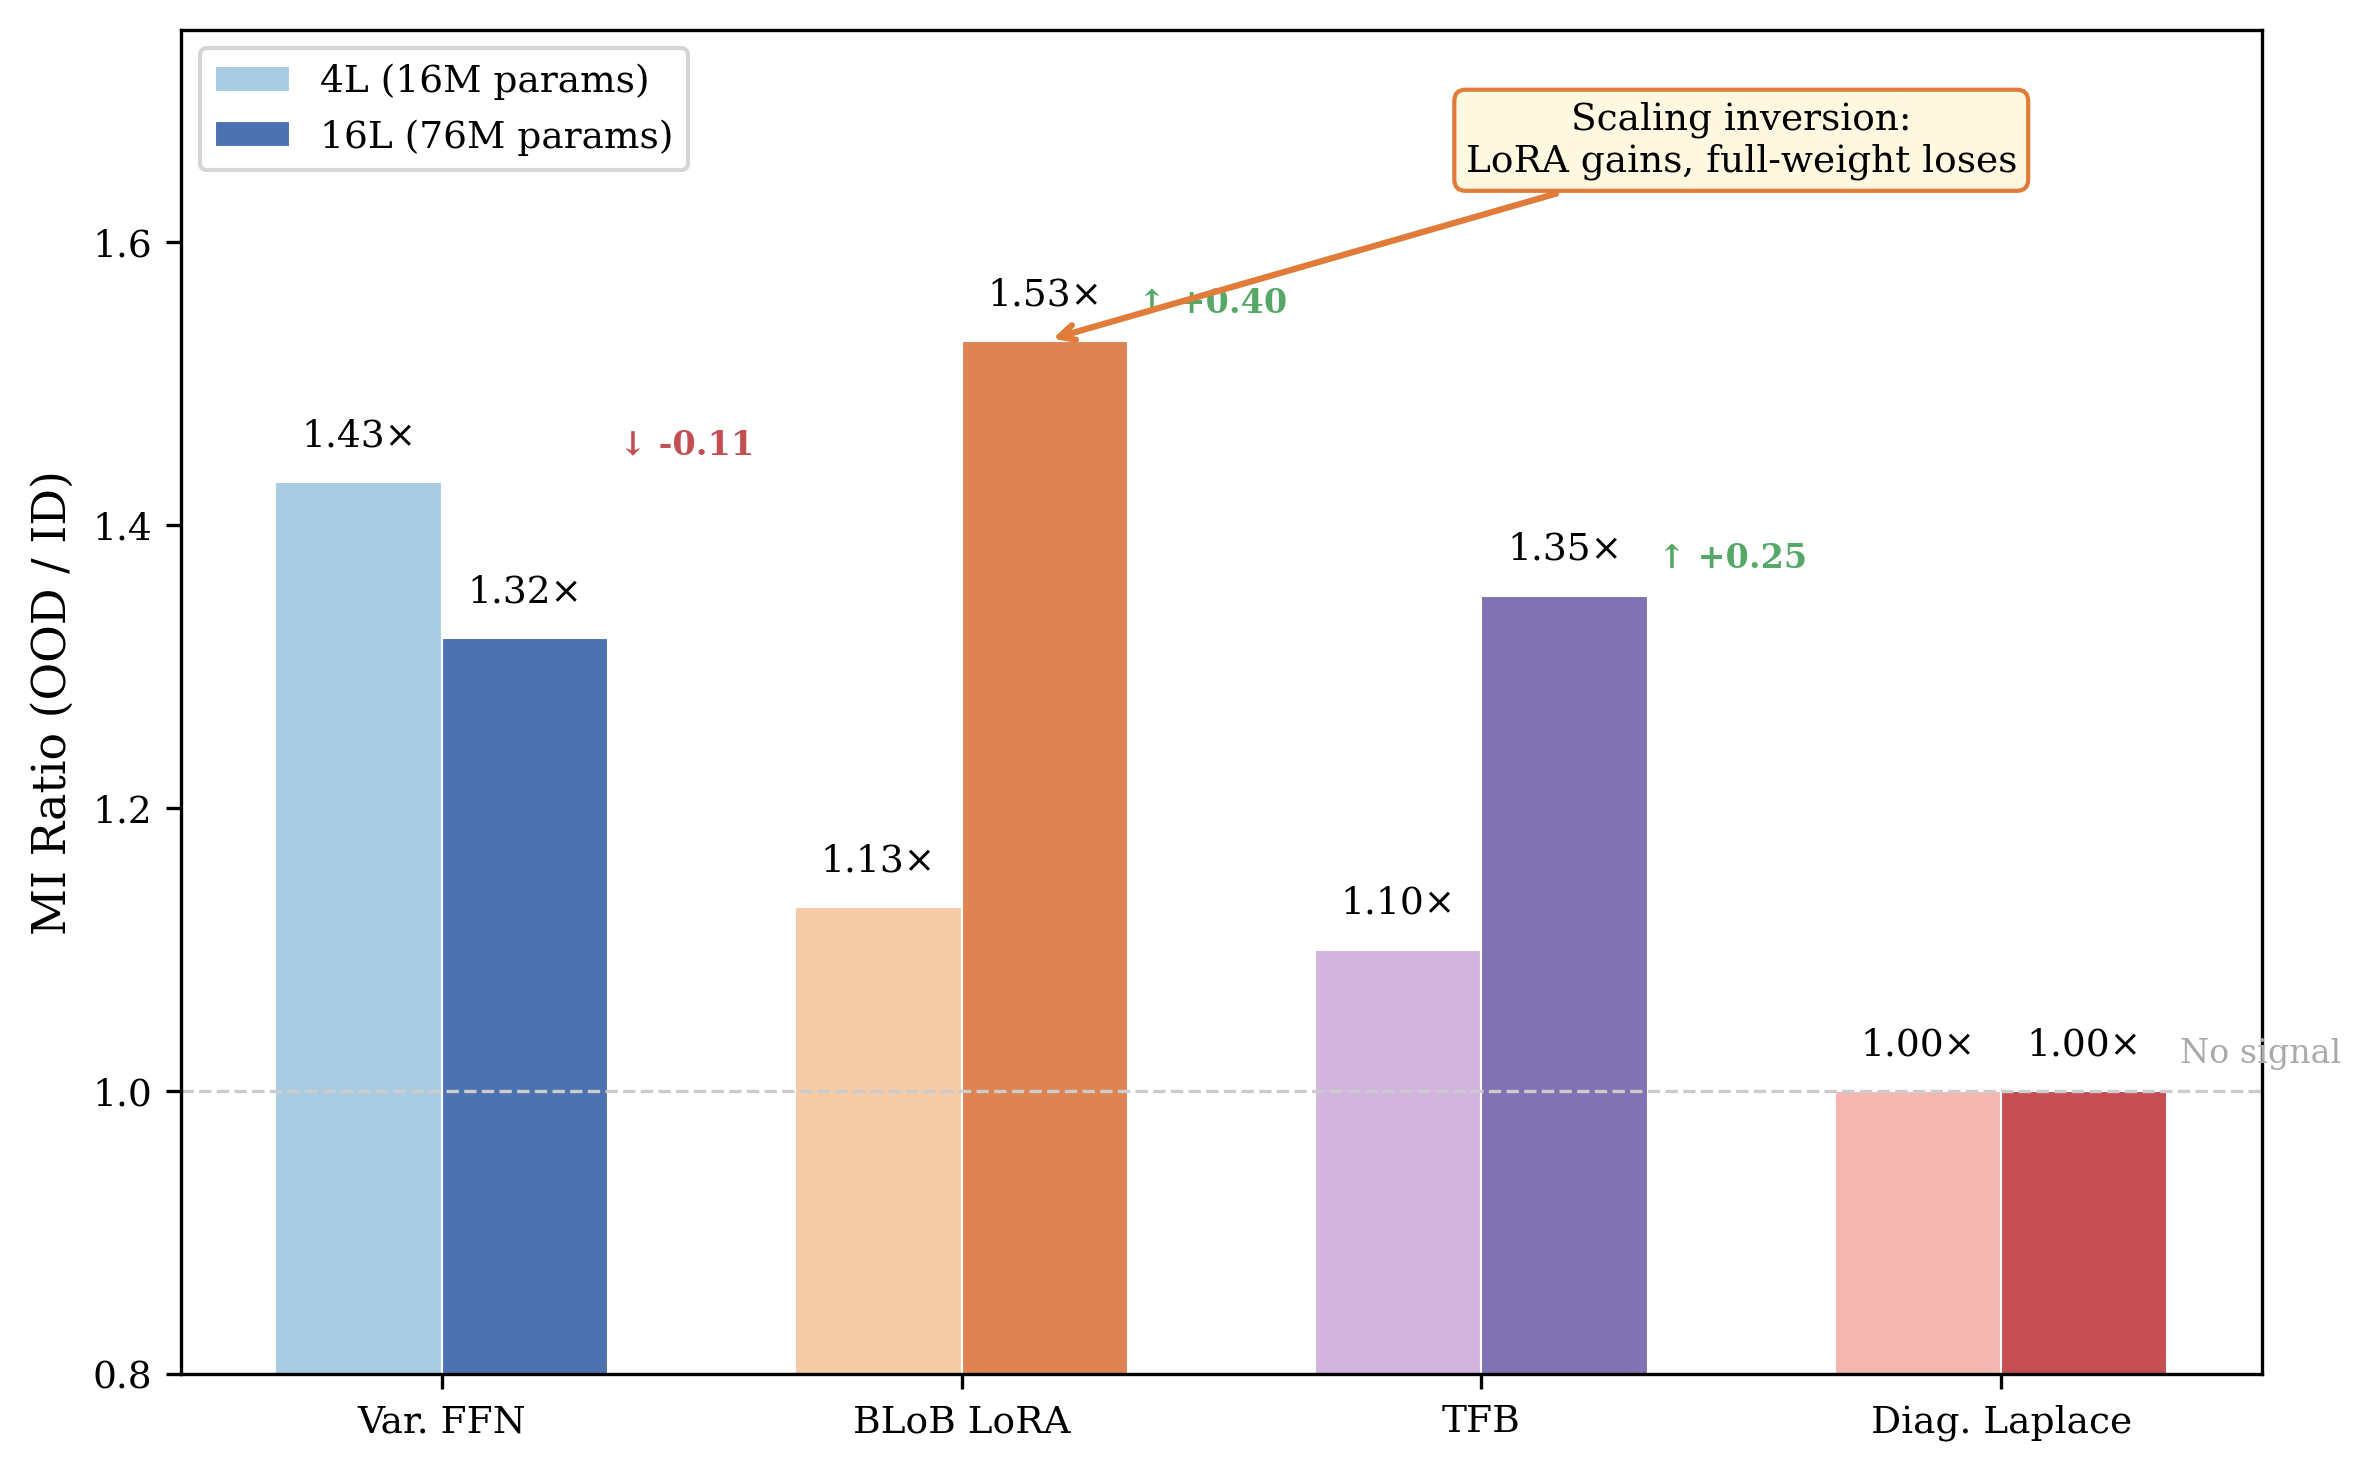
\includegraphics[width=0.85\textwidth]{fig7_scaling_inversion.png}
\caption{Scaling inversion: MI ratio at 4L (19M params) vs.\ 16L (76M params). At 4L, full-weight variational dominates; at 16L, LoRA methods overtake it---a reversal that suggests LoRA's constrained subspace becomes more beneficial as model size grows.}
\label{fig:scaling-inversion}
\end{figure}

\paragraph{LoRA vs.\ full-weight: an observational comparison.}
LoRA-based methods (BLoB, TFB) achieved stronger OOD detection than full-weight variational inference in our experiments (AUROC 0.909--0.917 vs.\ 0.874). However, this comparison is confounded by at least three factors: (1)~\textit{training procedure}---variational FFN trains the entire model from scratch with ELBO, while LoRA methods fine-tune adapters on a pre-trained deterministic backbone; (2)~\textit{backbone quality}---LoRA methods inherit a well-converged base model (ppl=14.3), while full-weight variational must learn representations and posteriors jointly (ppl=21.9); (3)~\textit{parameter count}---1.97M vs.\ 33.6M Bayesian parameters. One hypothesis is that LoRA's rank-16 subspace constrains posteriors to directions that matter for adaptation, producing more meaningful weight disagreement. But disentangling this subspace effect from the training-procedure and backbone-quality confounds requires ablations (e.g., variational fine-tuning on the pre-trained backbone, or BLoB LoRA from random initialization) that we leave to future work.

\paragraph{Diagonal Laplace: a hypothesis for the failure.}
Diagonal Laplace approximates the posterior covariance as the inverse of the diagonal Fisher information matrix. We observe that at convergence, the per-parameter Fisher values are near-zero for our well-trained language models---the loss landscape appears flat in most coordinate directions. We hypothesize that this produces an overly diffuse posterior that generates no meaningful prediction disagreement. The failure is consistent across full weights (33.6M params) and LoRA weights (1.97M params) at both 4L and 16L scale, suggesting the pattern may be general for diagonal Laplace on language models---though we note this does not extend to KFAC or full-Hessian variants, which capture off-diagonal curvature.

\begin{figure}[t]
\centering
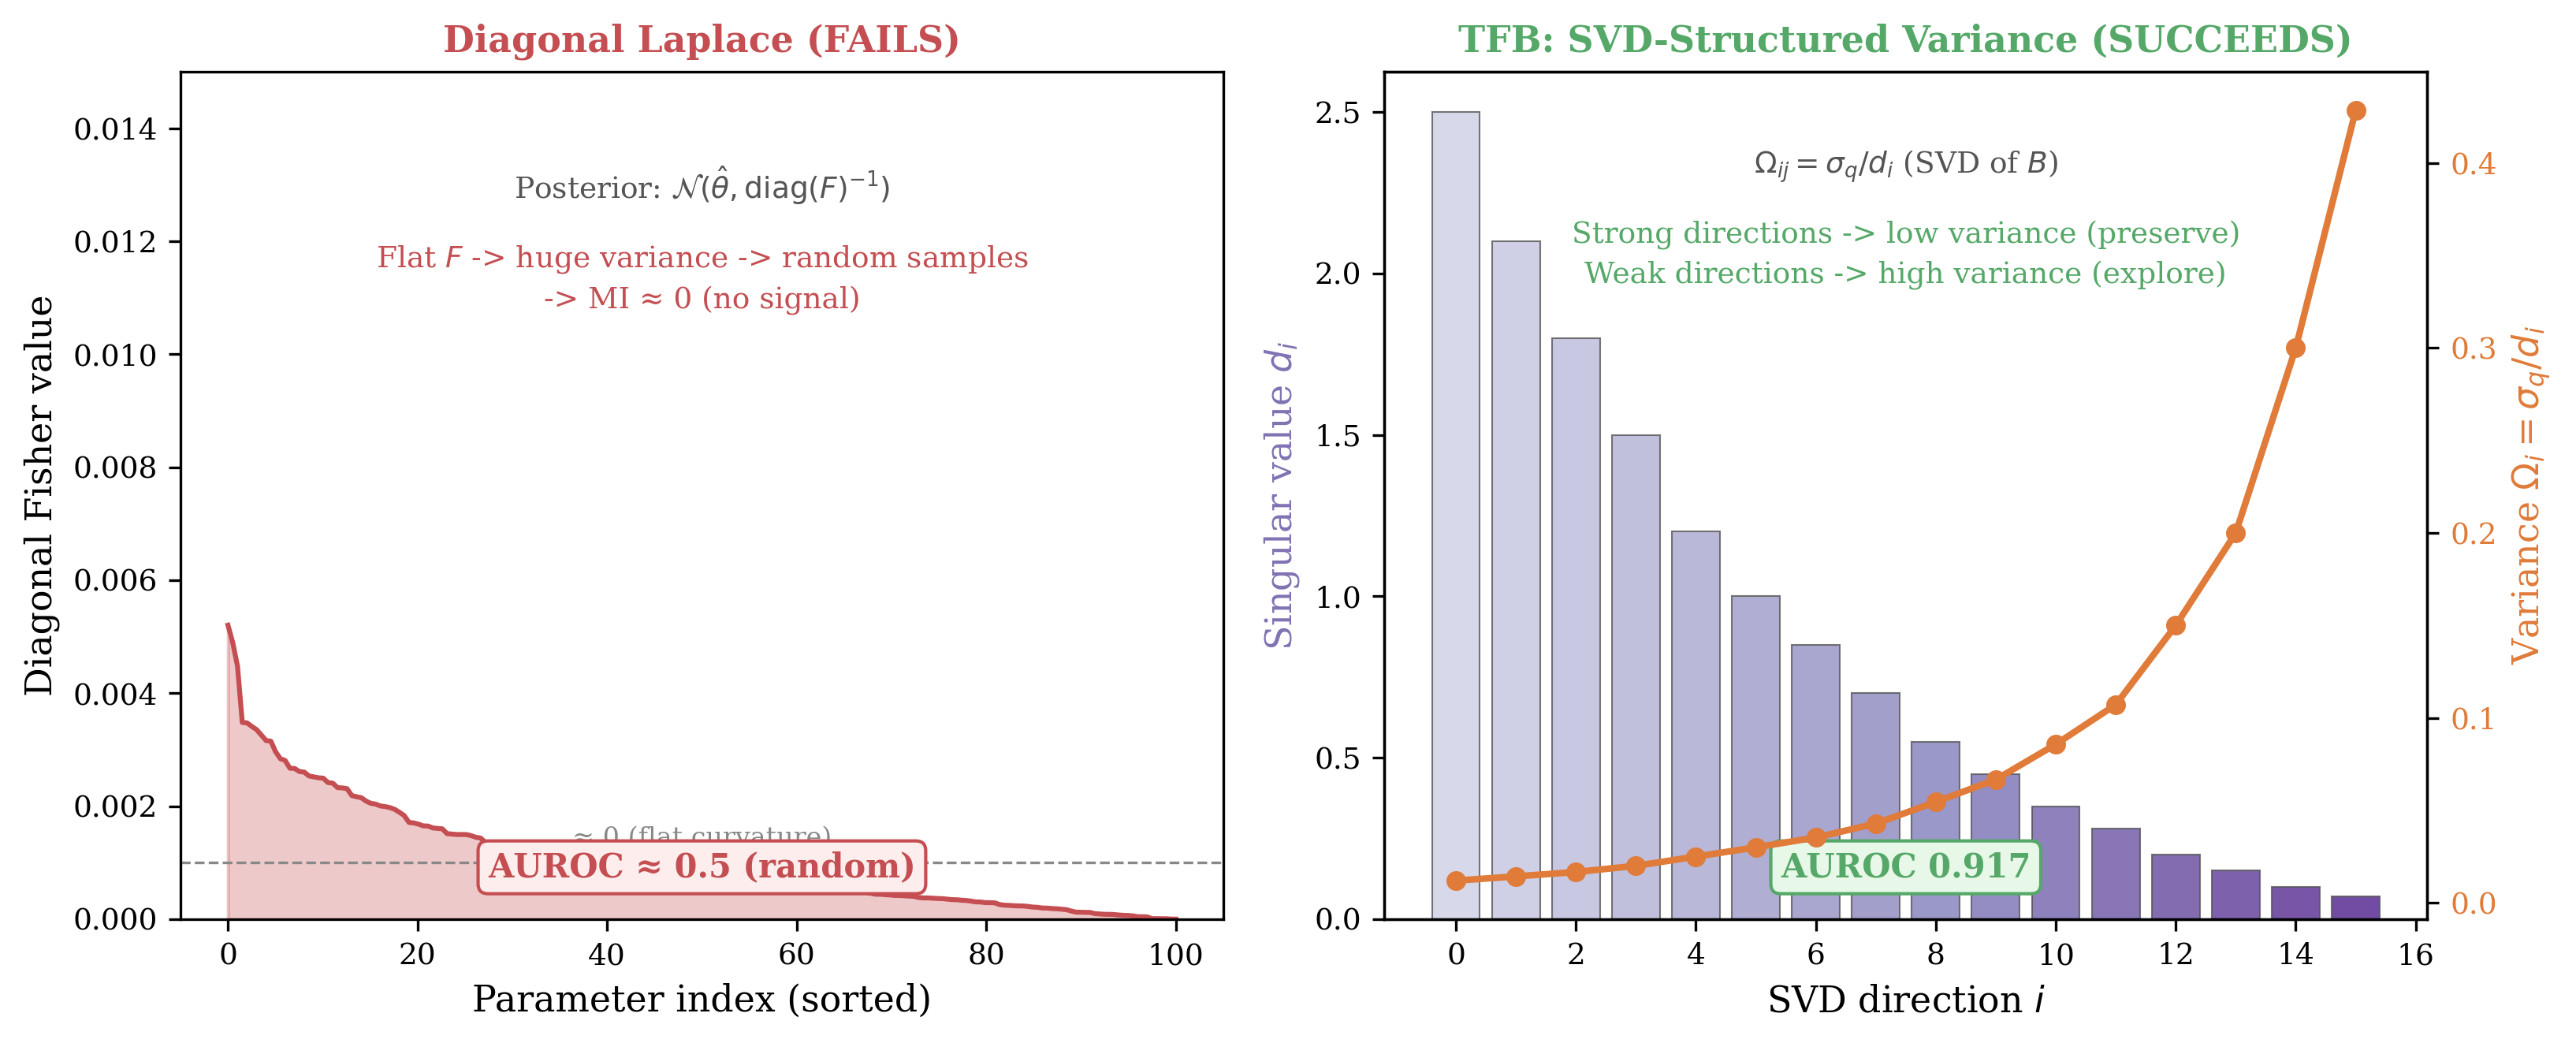
\includegraphics[width=0.85\textwidth]{fig4_tfb_vs_laplace.png}
\caption{Why post-hoc variance structure matters. TFB (left) derives variance from SVD of the $B$ matrix---singular values encode geometric structure of the LoRA subspace, remaining informative at convergence. Diagonal Laplace (right) uses Fisher curvature, which is flat at convergence for well-trained LMs, producing a posterior with no directional preference.}
\label{fig:tfb-vs-laplace}
\end{figure}

\paragraph{TFB vs.\ diagonal Laplace: a possible explanation.}
Both are post-hoc methods operating on LoRA parameters, yet TFB succeeds (AUROC 0.917) where diagonal Laplace fails (0.494). The key difference appears to be variance structure: diagonal Laplace uses curvature (diagonal Fisher), which in our experiments carries no directional information at convergence. TFB uses SVD of the $B$ matrix, which captures the geometric structure of the LoRA subspace---singular values encode how much each direction contributes to the weight update. We conjecture that this geometric information, being independent of the loss landscape's curvature, remains informative at convergence. Testing this hypothesis would require comparing TFB's SVD-structured variance against alternative variance structures (e.g., random isotropic, Fisher-weighted).

\paragraph{MC Dropout as a competitive baseline.}
MC Dropout \citep{gal2016dropout}---enabling dropout at inference on the deterministic checkpoint---achieves AUROC 0.898 with zero extra training cost. Its confidence interval [0.877, 0.917] overlaps with BLoB LoRA [0.890, 0.925], meaning we cannot claim statistical significance for the trained method's advantage at this sample size. MC Dropout also achieves the best calibration (ECE=0.012) among all methods. This suggests that for applications where marginal AUROC gains are not critical, MC Dropout may be the most cost-effective choice.

\paragraph{Limitations.}
Our comparison is conducted at 76M parameters on a GPT-2-style architecture. Scaling behavior to billion-parameter models remains an open question, though ScalaBL \citep{samplawski2025scalable} reports positive results for Bayesian LoRA at 32B. We evaluate only autoregressive language modeling with domain-split OOD; other tasks (classification, QA) and OOD types (semantic shift, adversarial) may yield different rankings. Our diagonal Laplace negative result does not extend to KFAC or full-Hessian Laplace variants, which capture off-diagonal curvature---though these are computationally expensive at scale. The LoRA vs.\ full-weight comparison is observational; the three confounds listed above prevent causal attribution. All results are from single training runs---bootstrap CIs capture evaluation variance but not training variance.

% ============================================================================
\section{Conclusion}
\label{sec:conclusion}

In a controlled $2{\times}2$ comparison of Bayesian uncertainty methods for language models, LoRA-based approaches (BLoB and TFB) achieved the strongest OOD detection at 76M-parameter scale (AUROC 0.909--0.917 vs.\ 0.874 for full-weight variational), though this advantage may partly reflect differences in training procedure and backbone quality rather than parameterization alone. MC Dropout---a zero-cost baseline---proved surprisingly competitive (AUROC 0.898, overlapping CIs with BLoB). TFB is particularly notable: it achieves the best AUROC (0.917) with zero Bayesian training---only a 7-minute binary search on an existing LoRA checkpoint. Diagonal Laplace approximation fails consistently across all configurations.

For production deployment, we recommend: (1)~merged mean-weights for serving predictions (zero overhead---LoRA means fold into base weights, producing a standard dense model), (2)~$N{=}3$ MC sampling for uncertainty scoring when needed (50\,ms/sequence, 382\,MB VRAM, 97\% of full signal). For applications where marginal AUROC gains over MC Dropout are not critical, MC Dropout on any existing checkpoint offers the lowest-cost path to epistemic uncertainty.

% ============================================================================
\bibliographystyle{plainnat}
\bibliography{references}

\end{document}
